
\chapter{Evaluation}

\section{Verifying Stack Protection}
\label{sec:stack_prot_eval}
% Create an example program. Show that accessing another task's stack memory yields fault.


\begin{figure}[h]
	\centering
	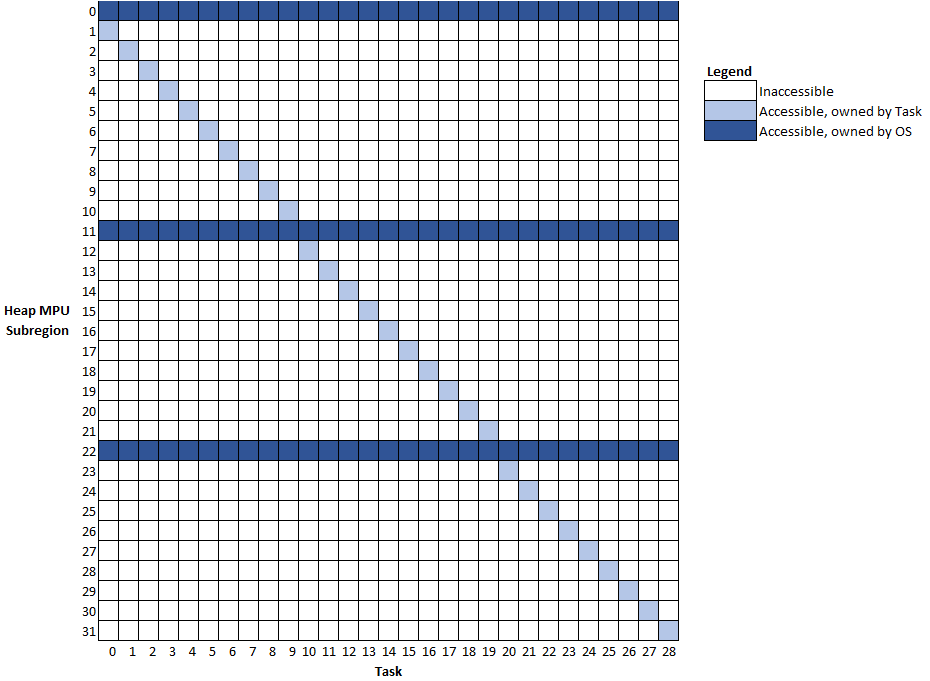
\includegraphics[width=\linewidth]{figs/task_access.png}
	\caption{Illustration of which tasks have access to which MPU subregions of the heap. This shows twenty-nine tasks, the maximum my solution can support with a 16KB heap.}
	\label{fig:task_access}
\end{figure}

Figure \ref{fig:task_access} shows which MPU subregions of the heap are accessible to which task for a system running twenty-nine tasks. Each task is allocated a unique subregion of its own, where its stack is located. Certain subregions (marked in gray) are owned by the OS (for storing TCBs) and are not accessible to any task.

In a simpler system, I can verify that accessing another task's stack generates a memory management fault. I spawn two OS tasks that both have access to a global integer pointer. Task A points the pointer to a local variable in its stack. Task B waits until Task A has done this and then tries to dereference the pointer to A's stack. Listing \ref{lst:stack_prot_test} shows the tasks for this test program.
\begin{lstlisting}[language=c, caption={Stack Protection Test Program}, captionpos=b, label={lst:stack_prot_test}, float]
Sema4Type sema;
volatile int *volatile task_a_stack = 0;

void TaskA(void) {
    volatile int x = 1;
    task_a_stack = &x;
    OS_bSignal(&sema); // Signal Task A to run
    while (1);
}

void TaskB(void) {
    OS_bWait(&sema); // Wait for Task B to signal
    volatile int z = *task_a_stack; // Should generate MPU fault
}
\end{lstlisting}

Indeed, upon running this program, one will see that a memory management fault is triggered immediately after dereferencing the pointer to Task A's stack. My design is successful at protecting a task's stack.

\section{Verifying Heap Protection}

\subsection{Reading/Writing Another Task's Heap Memory}

\begin{lstlisting}[language=c, caption={Heap Protection Test Program (Read/Write)}, captionpos=b, label={lst:heap_prot_test}, float]
    Sema4Type sema;
    volatile int *volatile task_a_heap = 0;
    
    void TaskA(void) {
        task_a_heap = (int*)Heap_Malloc(32);
        OS_bSignal(&sema); // Signal Task A to run
        while (1);
    }
    
    void TaskB(void) {
        OS_bWait(&sema); // Wait for Task B to signal
        volatile int z = *task_a_heap; // Should generate MPU fault
    }
\end{lstlisting}

We can modifying Listing \ref{lst:stack_prot_test} slightly to test heap protection as shown in Listing \ref{lst:heap_prot_test}. Rather than point \texttt{task\_a\_heap} at a stack variable, I assign it to the return value of Heap\_Malloc. Once again, Task B encounters a memory management fault upon dereferencing the pointer.

\subsection{Freeing Another Task's Heap Memory}

\begin{lstlisting}[language=c, caption={Heap Protection Test Program (Free)}, captionpos=b, label={lst:heap_free_test}, float]
    Sema4Type sema;
    volatile int *volatile task_a_heap = 0;
    
    void TaskA(void) {
        task_a_heap = (int*)Heap_Malloc(32);
        OS_bSignal(&sema); // Signal Task A to run
        while (1);
    }
    
    void TaskB(void) {
        OS_bWait(&sema); // Wait for Task B to signal
        Heap_Free(task_a_heap); // Should generate MPU fault
    }
\end{lstlisting}

With more small modifications, we can make sure that freeing another task's memory is similarly not allowed (Listing \ref{lst:heap_free_test}). Rather than dereference the pointer to Task A's heap memory, Task B passes it to Heap\_Free. Once again, this test succeeds and the access is denied by exception.

\section{Demonstrating Heap Flexibility}

In Section \ref{sec:stack_prot_eval} I showed that my solution supports up to twenty-nine tasks if each limits heap consumption to one subregion. However, my solution is flexible enough to allow greater consumption of the heap per-task. I will demonstrate the other extreme case where one task is able to allocate 14836 bytes at maximum on the heap (not including its stack memory).

\section{Measuring Context Switch Overhead}

\begin{table}[h]
\centering
\begin{tabular}{|l|l|}
\hline
\textbf{Config}                                                                        & \textbf{Context Switch Time} \\ \hline
No Memory Protection                                                                   & 1.792 microseconds           \\ \hline
\begin{tabular}[c]{@{}l@{}}Memory Protection with\\ Heavy Reconfiguration\end{tabular} & 7.167 microseconds           \\ \hline
\begin{tabular}[c]{@{}l@{}}Memory Protection with\\ Lite Reconfiguration\end{tabular}  & 6.25 microseconds           \\ \hline
\end{tabular}
\caption{Context switch duration.}
\label{tab:ctxsw}
\end{table}

In Table \ref{tab:ctxsw}, I measure the context switch duration for no memory protection, memory protection with heavy reconfiguration, and my design: memory protection with lite reconfiguration. The implementation with heavy reconfiguration fully initializes each of the four MPU regions of the heap during each context switch. This approximates a solution in which each task and/or process in the system maintains its own set of MPU regions which must be programmed into the MPU prior to running. This is much ``heavier'' reconfiguration than merely masking subregions of a constant region configuration as in my solution. The addition of memory protection does lengthen the context switch duration. That said, the context switch is shorter than it would otherwise be thanks to the use of subregions, which enable relatively light reconfiguration of the MPU during a context switch compared to heavier approaches. Lite reconfiguration yields a reduction in context switch duration of 12.8\%.
